\section{Ramp Rate Analysis} % 6.5

Like what we do in Section~\ref{section4.5} and in Section~\ref{section5.5}, we need to find the ramp rate in the emergency control. Results are as Table~\ref{6_5_risk}.


\begin{table*}[htbp]
\centering
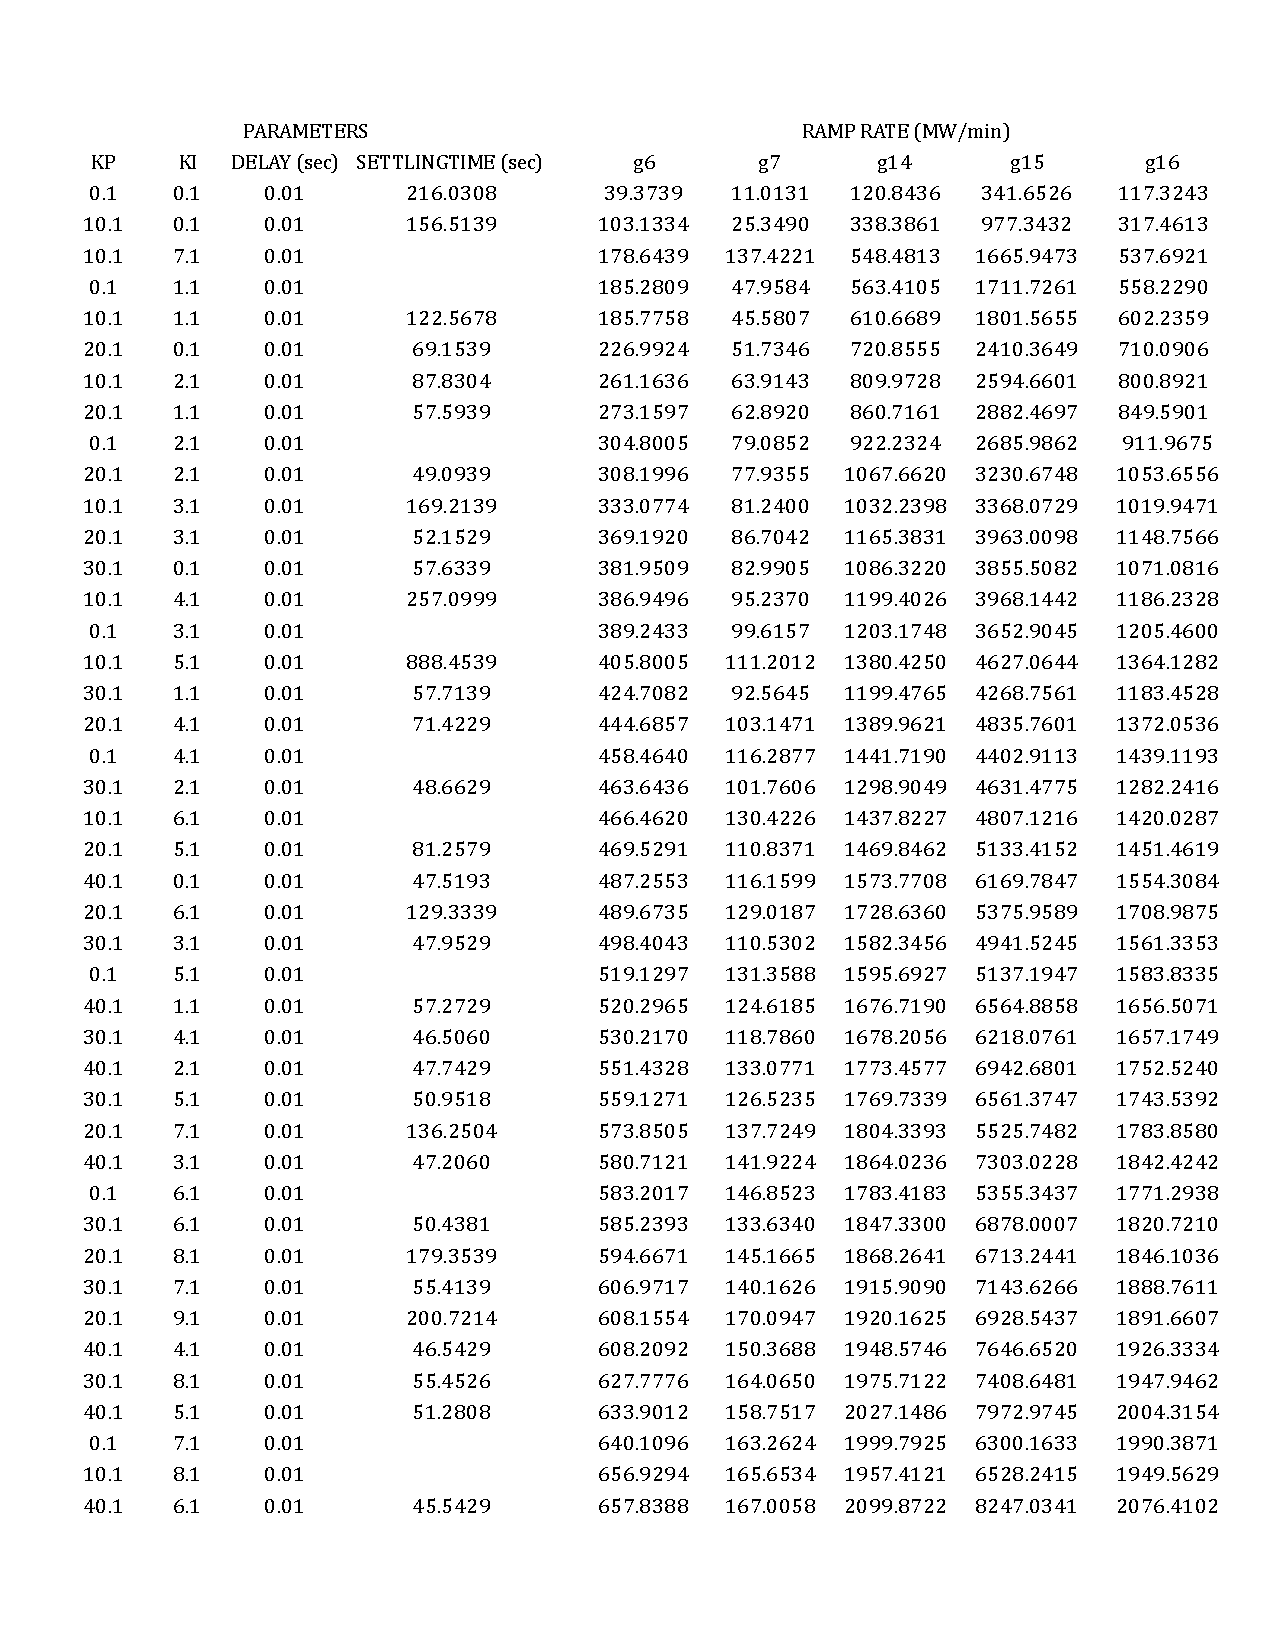
\includegraphics[width = \textwidth]{figure/6_5_risk.pdf}
\caption{Emergency Control: Some generators' real ramp rates, ranked by g6's ramp rate.}
\label{6_5_risk}
\end{table*}

Comparing Table~\ref{4_5_risk} and Table~\ref{6_5_risk}, we can find that the grid needs a larger ramp rate in the emergency control which shows that an alert state does weaken the stability of the system.